% Options for packages loaded elsewhere
\PassOptionsToPackage{unicode}{hyperref}
\PassOptionsToPackage{hyphens}{url}
\PassOptionsToPackage{dvipsnames,svgnames,x11names}{xcolor}
%
\documentclass[
  a4paper,
  DIV=11,
  numbers=noendperiod]{scrartcl}

\usepackage{amsmath,amssymb}
\usepackage{iftex}
\ifPDFTeX
  \usepackage[T1]{fontenc}
  \usepackage[utf8]{inputenc}
  \usepackage{textcomp} % provide euro and other symbols
\else % if luatex or xetex
  \usepackage{unicode-math}
  \defaultfontfeatures{Scale=MatchLowercase}
  \defaultfontfeatures[\rmfamily]{Ligatures=TeX,Scale=1}
\fi
\usepackage{lmodern}
\ifPDFTeX\else  
    % xetex/luatex font selection
\fi
% Use upquote if available, for straight quotes in verbatim environments
\IfFileExists{upquote.sty}{\usepackage{upquote}}{}
\IfFileExists{microtype.sty}{% use microtype if available
  \usepackage[]{microtype}
  \UseMicrotypeSet[protrusion]{basicmath} % disable protrusion for tt fonts
}{}
\makeatletter
\@ifundefined{KOMAClassName}{% if non-KOMA class
  \IfFileExists{parskip.sty}{%
    \usepackage{parskip}
  }{% else
    \setlength{\parindent}{0pt}
    \setlength{\parskip}{6pt plus 2pt minus 1pt}}
}{% if KOMA class
  \KOMAoptions{parskip=half}}
\makeatother
\usepackage{xcolor}
\setlength{\emergencystretch}{3em} % prevent overfull lines
\setcounter{secnumdepth}{5}
% Make \paragraph and \subparagraph free-standing
\ifx\paragraph\undefined\else
  \let\oldparagraph\paragraph
  \renewcommand{\paragraph}[1]{\oldparagraph{#1}\mbox{}}
\fi
\ifx\subparagraph\undefined\else
  \let\oldsubparagraph\subparagraph
  \renewcommand{\subparagraph}[1]{\oldsubparagraph{#1}\mbox{}}
\fi


\providecommand{\tightlist}{%
  \setlength{\itemsep}{0pt}\setlength{\parskip}{0pt}}\usepackage{longtable,booktabs,array}
\usepackage{calc} % for calculating minipage widths
% Correct order of tables after \paragraph or \subparagraph
\usepackage{etoolbox}
\makeatletter
\patchcmd\longtable{\par}{\if@noskipsec\mbox{}\fi\par}{}{}
\makeatother
% Allow footnotes in longtable head/foot
\IfFileExists{footnotehyper.sty}{\usepackage{footnotehyper}}{\usepackage{footnote}}
\makesavenoteenv{longtable}
\usepackage{graphicx}
\makeatletter
\def\maxwidth{\ifdim\Gin@nat@width>\linewidth\linewidth\else\Gin@nat@width\fi}
\def\maxheight{\ifdim\Gin@nat@height>\textheight\textheight\else\Gin@nat@height\fi}
\makeatother
% Scale images if necessary, so that they will not overflow the page
% margins by default, and it is still possible to overwrite the defaults
% using explicit options in \includegraphics[width, height, ...]{}
\setkeys{Gin}{width=\maxwidth,height=\maxheight,keepaspectratio}
% Set default figure placement to htbp
\makeatletter
\def\fps@figure{htbp}
\makeatother

\usepackage{booktabs}
\usepackage{longtable}
\usepackage{array}
\usepackage{multirow}
\usepackage{wrapfig}
\usepackage{float}
\usepackage{colortbl}
\usepackage{pdflscape}
\usepackage{tabu}
\usepackage{threeparttable}
\usepackage{threeparttablex}
\usepackage[normalem]{ulem}
\usepackage{makecell}
\usepackage{xcolor}
\KOMAoption{captions}{tableheading}
\makeatletter
\makeatother
\makeatletter
\makeatother
\makeatletter
\@ifpackageloaded{caption}{}{\usepackage{caption}}
\AtBeginDocument{%
\ifdefined\contentsname
  \renewcommand*\contentsname{Table of contents}
\else
  \newcommand\contentsname{Table of contents}
\fi
\ifdefined\listfigurename
  \renewcommand*\listfigurename{List of Figures}
\else
  \newcommand\listfigurename{List of Figures}
\fi
\ifdefined\listtablename
  \renewcommand*\listtablename{List of Tables}
\else
  \newcommand\listtablename{List of Tables}
\fi
\ifdefined\figurename
  \renewcommand*\figurename{Figure}
\else
  \newcommand\figurename{Figure}
\fi
\ifdefined\tablename
  \renewcommand*\tablename{Table}
\else
  \newcommand\tablename{Table}
\fi
}
\@ifpackageloaded{float}{}{\usepackage{float}}
\floatstyle{ruled}
\@ifundefined{c@chapter}{\newfloat{codelisting}{h}{lop}}{\newfloat{codelisting}{h}{lop}[chapter]}
\floatname{codelisting}{Listing}
\newcommand*\listoflistings{\listof{codelisting}{List of Listings}}
\makeatother
\makeatletter
\@ifpackageloaded{caption}{}{\usepackage{caption}}
\@ifpackageloaded{subcaption}{}{\usepackage{subcaption}}
\makeatother
\makeatletter
\@ifpackageloaded{tcolorbox}{}{\usepackage[skins,breakable]{tcolorbox}}
\makeatother
\makeatletter
\@ifundefined{shadecolor}{\definecolor{shadecolor}{rgb}{.97, .97, .97}}
\makeatother
\makeatletter
\makeatother
\makeatletter
\makeatother
\ifLuaTeX
  \usepackage{selnolig}  % disable illegal ligatures
\fi
\IfFileExists{bookmark.sty}{\usepackage{bookmark}}{\usepackage{hyperref}}
\IfFileExists{xurl.sty}{\usepackage{xurl}}{} % add URL line breaks if available
\urlstyle{same} % disable monospaced font for URLs
\hypersetup{
  pdftitle={Regional Inequalities and economic growth; cross section and times series analysis},
  pdfauthor={Anine Therese Karlsen \& Mona Lisa Jones},
  colorlinks=true,
  linkcolor={blue},
  filecolor={Maroon},
  citecolor={Blue},
  urlcolor={Blue},
  pdfcreator={LaTeX via pandoc}}

\title{Regional Inequalities and economic growth; cross section and
times series analysis}
\author{Anine Therese Karlsen \& Mona Lisa Jones}
\date{}

\begin{document}
\maketitle
\begin{abstract}
This assignment aims to acquire, process, and analyze sub-national GDP
and population data for a subset of European countries. Calculate GDP
per capita and explore regional inequity using various descriptive
statistics and visualizations.Furthermore examining the relationship
between regional development and inequality, employing cross sectional
estimation techniques for the year 2010.
\end{abstract}
\ifdefined\Shaded\renewenvironment{Shaded}{\begin{tcolorbox}[boxrule=0pt, sharp corners, frame hidden, borderline west={3pt}{0pt}{shadecolor}, breakable, interior hidden, enhanced]}{\end{tcolorbox}}\fi

\hypertarget{introduction}{%
\section{Introduction}\label{introduction}}

While national GDP and GDP per capita are vital indicators of a
country's aggregate economic health, they do not shed light on how
wealth or income is distributed among its residents. A high national GDP
can, paradoxically, coexist with pockets of regional deprivation
(\textbf{lessmann2017?}).

The truth of this statement becomes more evident when taking a closer
look at sub-national data. Regional wealth disparities are of prime
concern, especially when crafting policies for equitable growth
(\textbf{lessmann2017?}). A country's macro-level prosperity does not
automatically guarantee that all its regions partake equally in this
wealth. By studying smaller regions within a country, it is possible to
get a more nuanced narrative about the state of regional economic
disparities (\textbf{lessmann2017?}).

Using time series data and cross sectional observations we investigate
the GDP per capita and GINI trends in Portugal, France, Hungary,
Slovenia and Denmark in the time period 2000 to 2020. The aims is to
acquire, process, and analyze sub-national GDP and population data for a
subset of European countries. Calculate GDP per capita and explore
regional inequity using various descriptive statistics and
visualizations

\hypertarget{literature-review}{%
\section{Literature review}\label{literature-review}}

Regional growth and inequality have been important topics of research in
Europe for many years. In recent decades, the European Union has
implemented policies aimed at reducing regional disparities and
promoting economic growth across its member states. Furthermore, despite
these efforts, significant disparities in income and economic
development persist across regions in Europe (\textbf{lessmann2017?}).

When it comes to economic growth, several studies refer to numerous
influencing factors. (\textbf{gennaioli2014?}) and
(\textbf{crescenzi2012?}) states that regional growth, much like
national growth, is significantly influenced by geography and human
capital. Geography impacts trade, resource availability, and
susceptibility to natural events. Human capital, encompassing skills and
knowledge, drives innovation and productivity. Furthermore,
(\textbf{gennaioli2014?}) mentions that wealthier nations like Denmark
in our case, tend to experience faster regional convergence, suggesting
national prosperity aids regional growth (\textbf{gennaioli2014?}).
Convergence implies that poorer regions grow faster than richer ones,
gradually reducing disparities in wealth and income. Also referred to as
beta convergence in (\textbf{lessmann2017?}) paper.

In the context of Europe, and our selected countries we might expect to
see a wide variety of regional economic performances, especially within
Hungary and Slovakia and between the western European countries. Capital
market regulations also play a fundamental role, with effective
frameworks promoting quicker regional convergence
(\textbf{gennaioli2014?}). Taken this in to consideration we might
expect a faster growth rate after the joining of the EU in 2003 and
2004. That said the opening of the free labor market might also
influence the migration of labor in Slovakia and Hungary. Not to mention
the economic crisis hitting shortly after our eastern European countries
joined the union.

Whilst their recent EU membership might have posed certain challenges
for Eastern European countries during the financial crisis, it also
offered tools and resources that aided in their recovery in Slovakia and
Hungary. As to the western Europeans such as Denmark, Portugal and
France we expect to see a sharp decline in the economic growth.
Likewise, with the recent covid19 pandemic in terms of financial
aspects.

Regarding the effects of the economic crisis, another paper notes that
it led to a significant increase in regional unemployment rates across
Europe. Reporting some regions experiencing unemployment rates as high
as 30\% (\textbf{iammarino2019?}). The authors also discuss how the
crisis exposed the vulnerability of regions that were heavily reliant on
a single industry or sector, and how sheltered economies were better
able to weather the storm (\textbf{iammarino2019?}). Another affect that
surprised us was that the economic crisis led to increase inequality.
The study ``\emph{the effects of financial crisis on regional
inequality}'' indicate any type of financial crisis results in higher
income inequality (\textbf{nguyen2022?}).

(\textbf{lessmann2017?}) regional inequality study address the
importance of studying regional inequality. In particular, its potential
consequences, such as political tensions that can undermine social and
political stability (\textbf{lessmann2017?}). The paper also discusses
the relationship between regional inequality and personal income
inequality and conflict risk. Furthermore, the paper provides us with
insights into the inverted U-shaped relationship between regional
inequality and the level of economic development in different country
groups (\textbf{lessmann2017?}). The inverted U-shape also referred to
as Kuznets Curve suggests that as an economy develops, regional
inequality initially rises, reaches a peak, and then starts to decline.
(\textbf{lessmann2017?}) paper also finds that there is an N-shaped
relationship between regional inequality and economic development, which
means that regional inequality increases again after the inverted
U-shaped pattern has been completed (\textbf{lessmann2017?}).

Lastly, (\textbf{iammarino2019?}) discusses regional inequalities in
European countries. It presents evidence that inter-regional inequality
has been increasing in the European Union since the turn of the
millennium. The authors argue that this is due to the existence of
several groups of regional economies in Europe that are structurally
very different from one another (\textbf{iammarino2019?}). Additionally,
the authors argue that there are some countries in the EU that are more
evenly developed than others, and that a map of under performance or
over-performance means less in a high-income but evenly developed
country, such as in Denmark in our case (\textbf{iammarino2019?}). On
the other hand, France has been a subject of discussion and policymaking
for many years, regarding its pockets of extreme wealth. (finner ikke
kilde)

\hypertarget{data}{%
\section{Data}\label{data}}

Trough Eurostat, we download the datasets nama\_10r\_3gdp and
demo\_r\_pjanggr3 as csv files and filted the data by our preferences
before downloading it. Furthermore, we filtered the dataset by choosing
the years 2000 to 2020. Then, we selected the NUTS 3 region for
Portugal, France, Hungary, Slovakia and Denmark. Finally, we specified
the data to be in million Euro.

\hypertarget{gdp}{%
\subsubsection{GDP}\label{gdp}}

The GDP dataset provides insights into GDP at regional level using the
NUTS classification system. It furnishes GDP values in both current
prices and adjusted for inflation, with figures given in purchasing
power standards (PPS) to account for price level differences between
countries. The data is mostly structured by year and region
(\textbf{eurostat2023?}).

The GDP at market prices represents the final result of production
activities of resident producer units within a region or nation. It is
calculated as the sum of the gross value added across various
institutional sectors or industries. Furthermore, augmented by taxes and
reduced by subsidies on products (which are not allocated to specific
sectors or industries) (\textbf{eurostat2023c?}). This also balances out
in the total economy production account. In terms of methodology, while
national accounts compile GDP from the expenditure side, regional
accounts don't adopt this approach due to the complexities of accurately
mapping inter-regional flows of goods and services.

The different measures for the regional GDP are absolute figures in €
and Purchasing Power Standards (PPS), figures per inhabitant and
relative data compared to the EU Member States average
(\textbf{eurostat2023c?}).

\hypertarget{population}{%
\subsubsection{Population}\label{population}}

Eurostat's records annual population data with NUTS classification. Our
dataset includes information on births, deaths, net migration, and may
also include demographic information on age and gender. Displayed in a
year-by-region format, with yearly interval updates
(\textbf{eurostat2023a?}).

Eurostat's primary source for yearly demographic data at the regional
level stems from the Unified Demography (Unidemo) project. The project
covers 37 countries and is the central repository for demographic and
migration-related data (\textbf{eurostat2023a?}). As well as, specific
metrics gathered under UNIDEMO encompass population counts at the close
of the calendar year and events such as births and deaths occurring
within that year (\textbf{eurostat2023a?}). Additionally, data on
marriages, divorces, and migration flows are recorded .

For the purpose of this research, the demographic data references the
NUTS 2016 classification, which provides a detailed breakdown of the
European Union's territory (\textbf{eurostat2021?}).

\hypertarget{nuts-classification}{%
\subsubsection{NUTS classification}\label{nuts-classification}}

The Nomenclature of Territorial Units for Statistics (NUTS) offers a
stratified system to segment the economic territory of the EU and UK to
facilitate the consistent collection and harmonization of regional
statistics across Europe. The NUTS regions range from NUTS 0 Country
level to NUTS 3 small units such as municipalities level
(\textbf{eurostat2023a?}). ~

\hypertarget{econometric-approach}{%
\section{Econometric Approach}\label{econometric-approach}}

In this part we will report and interpret different types of essential
descriptive statistics. Measuring regional income inequality is
challenging due to heterogeneity of regions (\textbf{lessmann2017?}).
The number of regions in our data set varies largely in size and
population. Since the focus of this paper is purely growth and changes
in inequities over time, the variations of size and population density
becomes a minor issue because the country-level territorial
heterogeneity is fixed (\textbf{lessmann2017?}).

``Interest in income inequality has led to the development of several
ways of measuring it. Two types of measures are of interest in this
paper----static and dynamic. \emph{Static measures} provide a snapshot
(cross sectional) of these inequalities at a point of time whereas the
dynamic \emph{measures capture historical trends} (Paneldata)\emph{.}''
(\textbf{wooldridge2020?})

By using figures, we can visualize the GDP per capita, and look at how
it varies among the different regions. In these figures, a line
represent one NUTS 3 region.

\hypertarget{descriptive-statistics}{%
\subsubsection{Descriptive statistics}\label{descriptive-statistics}}

\textbf{Mean}

We calculate the mean to provide a representative value for the dataset,
facilitating understanding of its central tendency and serving as a
benchmark against which deviations and anomalies can be assessed, in
later steps when building and interpreting regression models
(\textbf{wooldridge2020?}).

\textbf{MMR}

Comparing the GRDP (gross regional domestic product) per capita of the
region with the highest income to the region with the lowest income
(minimum per capita GRDP) provides a measure of the range of these
disparities. If this measure is small (close to 1), then it would mean
that the different regions have relatively equal incomes
(\textbf{wooldridge2020?}). If this measure is large, then the
interpretation is more problematic, as it does not tell us if the high
ratio is due to substantial variation in the distribution of per capita
GDRPs or the presence of outliers. Nevertheless, maximum to minimum
ratio (MMR) provides a quick, easy to comprehend, and politically
powerful measure of regional income inequality.

\textbf{Standard diviation (SD)}

Calculating SD to quantify the dispersion or variability of a data set
around its mean. Helping us assess the degree of uncertainty,
variability, or risk associated with an economic variable or parameter,
which is crucial for understanding the reliability of estimations and
predictions (\textbf{wooldridge2020?}).

\textbf{Median}

The median serves as a robust measure of central tendency, especially
when a dataset may have outliers or is skewed. Unlike the mean, the
median is not influenced by extreme values and, thus, can provide a
clearer picture of the ``typical'' value in situations where the data
distribution is not symmetrical (\textbf{wooldridge2020?}).

\hypertarget{time-series-panel-data}{%
\subsubsection{\texorpdfstring{\textbf{Time series (Panel
data)}}{Time series (Panel data)}}\label{time-series-panel-data}}

\hypertarget{cross-sectional-analysis}{%
\subsubsection{Cross sectional
analysis}\label{cross-sectional-analysis}}

\hypertarget{simple-linear-regression}{%
\subsubsection{Simple linear
regression}\label{simple-linear-regression}}

\hypertarget{multiple-linear-regression}{%
\subsubsection{Multiple linear
regression}\label{multiple-linear-regression}}

\hypertarget{part-1a-sub-national-gdp-and-gdp-per-capita}{%
\section{Part 1A: Sub-national GDP and GDP per
Capita}\label{part-1a-sub-national-gdp-and-gdp-per-capita}}

\hypertarget{gdp-per-capita-calculation}{%
\subsection{GDP per Capita
Calculation}\label{gdp-per-capita-calculation}}

The formula for calculating GDP per Capita is as follows:

\(y_i=GDP_i/population_i\)

After calculating the GDP per capita for all NUTS 3 regions within the
chosen countries, we can see that there is a large spread between the
figures for the various regions. We want to look at regional inequity;
in order to do this in a valuable way, countries are divide.
Furthermore, gaining important insights on regional differences and
utilize. Later to discuss national policy on equity and sustainable
economic development in regions.

\hypertarget{portugal}{%
\subsubsection{Portugal}\label{portugal}}

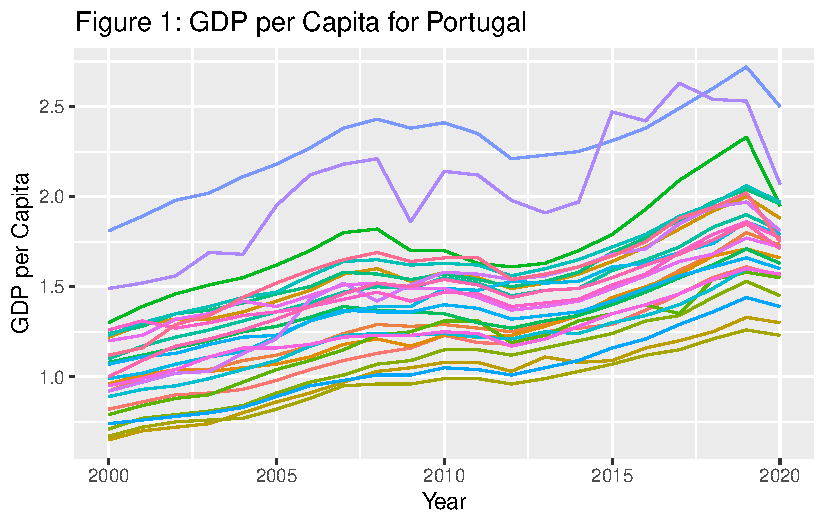
\includegraphics{MSB104_GR_1_Final_Assignment_research_article_files/figure-pdf/unnamed-chunk-7-1.pdf}

\begin{verbatim}
        GDP_per_capita
mean         1.4185524
median       1.3900000
std_dev      0.3702905
minimum      0.6500000
maximum      2.7200000
\end{verbatim}

By looking at figure for Portugal, we can see that the GDP per capita in
Portugal's regions appears to be fairly consistent. There is however
some regional variability. We can see that the regions around the big
cities like Lisbon have a higher GDP per capita compared to some more
rural areas. Since Lisbon is the capital of Portugal, there is probably
a higher concentration of industries, making it a economic center (which
again makes the GDP per capita higher).

To continue, we can see that the mean is a little higher that the
median, something that might indicate that regions like Lisbon are
pulling up the average. If we compare the standard derivation for
Portugal with the other countries, we'll see that is fairly low in
comparison. This might mean that there is not a lot of variability
between the GDP per capita across different regions in Portugal. The gap
between minimum and maximum is also low compared to other countries,
something that'll also show us that the economic disparity in Portugal
might not be as high as it is in other countries.

\hypertarget{france}{%
\subsubsection{France}\label{france}}

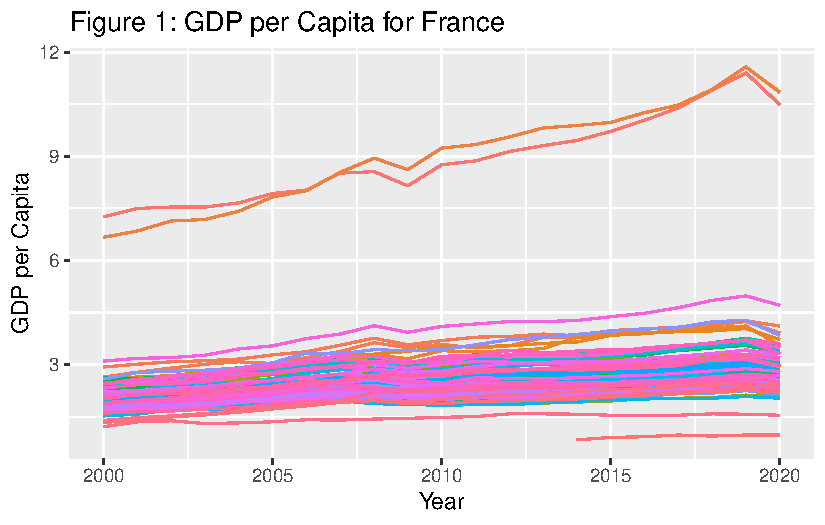
\includegraphics{MSB104_GR_1_Final_Assignment_research_article_files/figure-pdf/unnamed-chunk-10-1.pdf}

\begin{verbatim}
        GDP_per_capita
mean          2.630444
median        2.440000
std_dev       1.053767
minimum       0.830000
maximum      11.580000
\end{verbatim}

When looking at the figure for France, we see some regions have a much
higher GDP per capita compared to the other regions. The regions with
the highest GDP per capita for all years is the île-de-France region,
one that also includes Paris. This significant difference between the
regions with the highest GDP per capita and the lowest, shows us that
there is a high concentration of economic activity and wealth in a few
urban regions. Similar to Portugal, we see differences between urban and
rural regions.

Just as in Portugal, there is also a higher mean in France as well. On
the contary the data in France has higher standard derivation, and the
difference between minimum and maximum is larger. This strengthens
earlier figures showing, some regions having a high concentration of
wealth.

\hypertarget{hungary}{%
\subsubsection{Hungary}\label{hungary}}

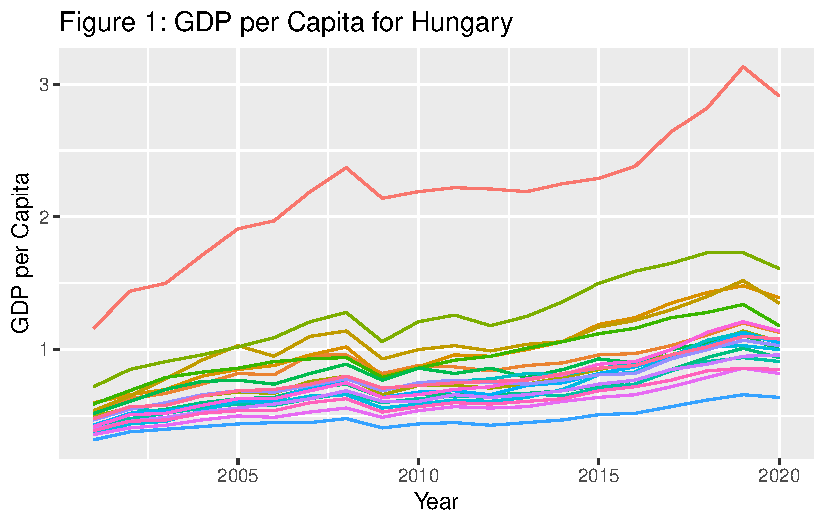
\includegraphics{MSB104_GR_1_Final_Assignment_research_article_files/figure-pdf/unnamed-chunk-13-1.pdf}

\begin{verbatim}
        GDP_per_capita
mean         0.8598000
median       0.7650000
std_dev      0.4059723
minimum      0.3200000
maximum      3.1300000
\end{verbatim}

In Hungary, most of the regions have similar GDP per Capita. One region
that sticks out by having a higher value, is the region of Budapest, the
capital.

This case also record the mean as higher vale than the median, high
standard derivation, and a large gap between minimum and maximum.

\hypertarget{slovakia}{%
\subsubsection{Slovakia}\label{slovakia}}

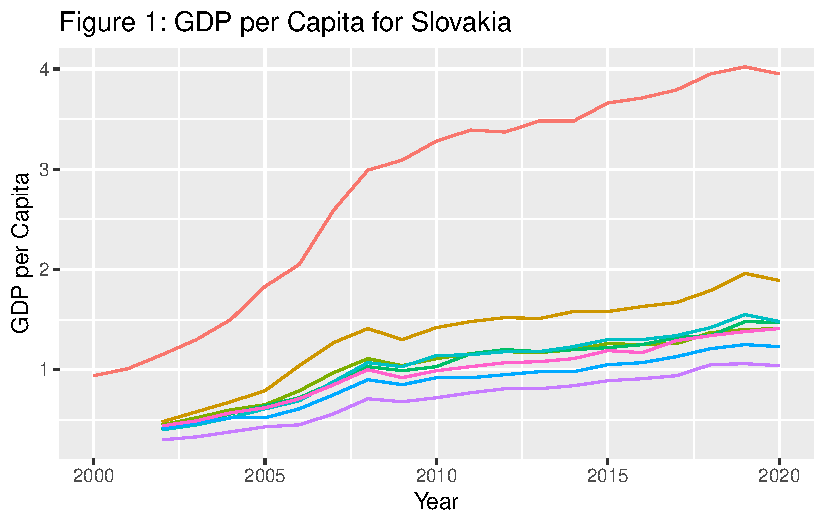
\includegraphics{MSB104_GR_1_Final_Assignment_research_article_files/figure-pdf/unnamed-chunk-16-1.pdf}

\begin{verbatim}
        GDP_per_capita
mean         1.2501948
median       1.0950000
std_dev      0.8018259
minimum      0.3000000
maximum      4.0200000
\end{verbatim}

Additionally, Slovakia, also have one region with much higher GDP per
capita than the rest of the regions. This region is Bratislava, which is
the biggest city and the capital, something that might point to this
city being the economic centre of Slovakia as well.

Slovakia follows the trend with higher mean than the median, and a large
gap between minimum and maximum. In addition, the standard derivation is
significantly high, meaning that there is some regions (or one region in
this case) that is further away from the rest of the regions in terms of
economic development.

\hypertarget{denmark}{%
\subsubsection{Denmark}\label{denmark}}

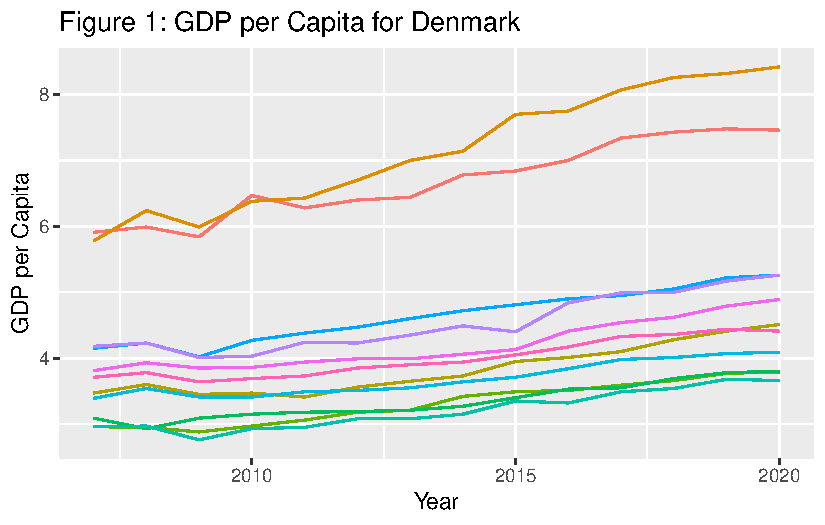
\includegraphics{MSB104_GR_1_Final_Assignment_research_article_files/figure-pdf/unnamed-chunk-19-1.pdf}

\begin{verbatim}
        GDP_per_capita
mean          4.419221
median        4.000000
std_dev       1.343933
minimum       2.760000
maximum       8.420000
\end{verbatim}

Lastly, we see similar pattern in Denmark, with the capital Copenhagen
being one of the regions with the highest GDP per capita.

Whith mean higher than the median, showing that regions like Copenhagen
possible dragging the mean up by population volume.

\hypertarget{part-1b-regional-inequity}{%
\section{Part 1B: Regional Inequity}\label{part-1b-regional-inequity}}

\hypertarget{gini-coefficient-calculation}{%
\subsection{Gini Coefficient
Calculation}\label{gini-coefficient-calculation}}

With the use of the NUTS3 GDP per capita data and this formula:

\(GINW_j=\frac{1}{2 \bar{y_j}} \sum_{i}^{n_j}\sum_{l}^{n_j}\frac{p_i}{P_j} \frac{p_l}{P_j} |y_i-y_l|\)

we will compute the population-weighted GDP Gini coefficient for each
European NUTS2 region in our assigned countries.

The gini coefficient can help us measure inequality in a distribution,
as is therefore a useful tool for us to use when we look at regional
inequity. The closer the gini coefficient is to 1, the bigger the
inequality is; a number closer to 0 equals equality. When looking at the
gini coefficient for NUTS 2 regions, we also get a better overview over
differences in income between different regions, and it also makes it
easier to find the reasons as to why there is a difference between the
regions (\textbf{hasell2023?}).

After calculating the gini coefficients, we can see that there are some
similarities to the data we got from GDP per capita for NUTS 3 regions.
In order to see these similarities better, as well as look for other
important aspects that can be provided trough the calculations, we will
visualize the data in three different ways.

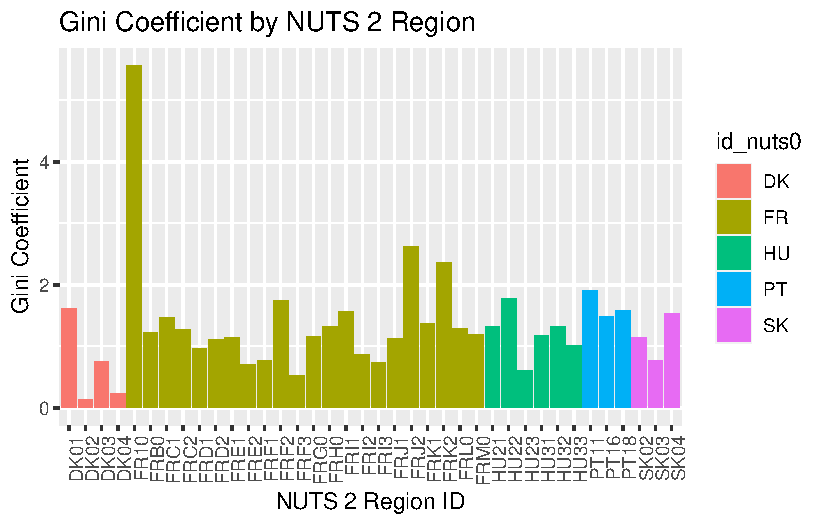
\includegraphics{MSB104_GR_1_Final_Assignment_research_article_files/figure-pdf/unnamed-chunk-23-1.pdf}

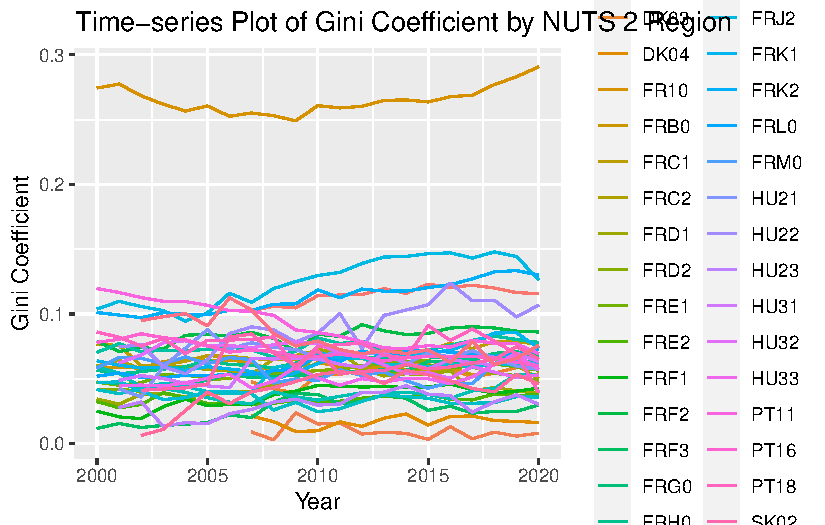
\includegraphics{MSB104_GR_1_Final_Assignment_research_article_files/figure-pdf/unnamed-chunk-24-1.pdf}

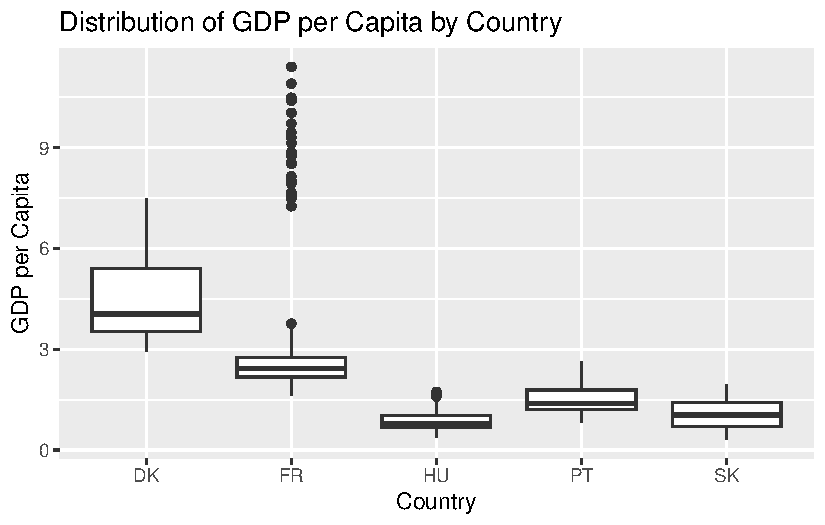
\includegraphics{MSB104_GR_1_Final_Assignment_research_article_files/figure-pdf/unnamed-chunk-25-1.pdf}

\hypertarget{part-2a-growth-and-inequity}{%
\section{Part 2A: Growth and
Inequity}\label{part-2a-growth-and-inequity}}

\hypertarget{data-acquisition}{%
\subsubsection{\texorpdfstring{\textbf{Data
acquisition}}{Data acquisition}}\label{data-acquisition}}

Firstly, the data is summerised for the year 2010 at the NUTS2 regional
level, focusing on economic metrics. Processing the dataset containing
the NUTS3 level. Thereafter, computing the total GDP and total
population for each NUTS2 region and year. Then, derive the GDP per
capita at the NUTS2 level by dividing the total GDP by the total
population again. Furthermore, narrowing down the dataset to
observations from the year 2010 where the Gini coefficient is positive.
Then adding, logarithmic transformations to linearize relationships or
to reduce the impact of extreme values.

The next step is making a data frame of NUTS2 2010 and grouping by NUTS0
country level variables, as well as allocating NUTS2 to selected
countries. Lastly presenting data in \textbf{table XXX} showing a count
of NUTS2 regions within each top-level region or country in the 2010
data.

\textbf{\#Esempel:Looking at the descriptive statistics we see in
average a very low level of inequality within all regions. Even at the
maximum inequality is modest with 0.35 spacial in comparison with other
countries, see for example Lessmann and Seidel
(\href{https://a10747-2033066.cluster215.canvas-user-content.com/courses/10747~22507/files/10747~2033066/course\%20files/html/Assignments_example.html?context_id=10747~22507\&context_type=Course\&download=1\&id=107470000002033066\&inline=1\#ref-lessmann2017regional}{2017})
for such a comparison.Studding the temporal component of our data we see
that most regions follow a common trend in there level of inequality
with modest changes over time. See for example the NUTS2 regions of
France in
\href{https://a10747-2033066.cluster215.canvas-user-content.com/courses/10747~22507/files/10747~2033066/course\%20files/html/Assignments_example.html?context_id=10747~22507\&context_type=Course\&download=1\&id=107470000002033066\&inline=1\#fig-regional_gini_time}{Figure~4}.
There are however some severe exceptions \ldots\#}

The next step is, estimating a Linear Regression for All Countries using
cross sectional data from 2010, NUTS2.

\hypertarget{cross-sectional-analysis-1}{%
\subsubsection{\texorpdfstring{\textbf{Cross Sectional
Analysis}}{Cross Sectional Analysis}}\label{cross-sectional-analysis-1}}

With cross-sectional data analysis we create a snapshot of the year
2010. Cross-sectional data is simpler to manage and interpret than
time-series or panel data. With data from only one time point, we avoid
complications arising from temporal dynamics. Cross-sectional data
allows for the comparison of different regions at the same time, which
can be crucial for identifying disparities or differences between the
regions (\textbf{wooldridge2020?}).

\hypertarget{simple-linear-regression-model}{%
\subsubsection{\texorpdfstring{\textbf{Simple linear regression
model}}{Simple linear regression model}}\label{simple-linear-regression-model}}

We use simple linear regression to model the relationship with the GINI
as the dependent variable and the natural logarithm of GDP per capita as
the independent variable. Capturing the relationship between regional
development and regional inequality for all regions in 2010.

\textbf{Model assumptions}

``The relationship between our dependent and independent variables is
linear, ensuring a clear and direct connection between them. Each
observation operates independently of the others, emphasizing the unique
contribution of every data point. Additionally, we expect
homoscedasticity, implying that the variance of the residuals remains
consistent regardless of the independent variable's level. It's also
crucial that, for any specified value of X, Y maintains a normal
distribution. And although more pertinent to multiple regression, it's
worth noting the absence of multicollinearity, ensuring that no two
predictors are closely correlated.''

\textbf{Model specification}

\textbf{\#\#\#Vis formel\#\#}

Y is the dependent variable (hva som perdikeres).

X is the independent variable (input).

β0\hspace{0pt} is the intercept.

β1\hspace{0pt} is the slope of the line.

ε represents the residuals or error in the prediction.

\begin{itemize}
\item
  \textbf{Intercept (}β0\hspace{0pt}): represents the value of Y when X
  is 0.

  \textbf{Slope (}β1\hspace{0pt}): Indicates the change in Y for a
  one-unit change in X.
\end{itemize}

``In linear regression, the objective is straightforward: determine the
line that best represents the observed data. Furthermore, this `goodness
of fit' line is characterized by coefficients β0\hspace{0pt} and β1,
which represent the intercept and slope, respectively
(\textbf{wooldridge2020?}). The optimal line is one that minimizes the
sum of the squared differences between the observed values and the
predictions made by the model (\textbf{wooldridge2020?}). This approach,
known as the Ordinary Least Squares (OLS), has a solid mathematical
foundation (\textbf{wooldridge2020?}). By taking the sum of these
squared differences and setting their partial derivatives with respect
to β0\hspace{0pt} and β1 to zero, we can derive the formula that give us
these coefficients. And once these coefficients are in hand, they
provide a direct equation for the line that best fits our data set
(\textbf{wooldridge2020?}). One of the strengths of OLS is its
closed-form solution, meaning we can directly compute the coefficients
from the data without iterative procedures (\textbf{wooldridge2020?}).
Moreover, under the foundamental assumptions of linear regression, OLS
stands out as the Best Linear Unbiased Estimator (BLUE), emphasizing its
reliability and efficiency in estimating the true underlying
relationship (\textbf{wooldridge2020?}).''

\hypertarget{individual-country-cases}{%
\subsubsection{Individual country
cases}\label{individual-country-cases}}

\hypertarget{portugal-1}{%
\paragraph{Portugal}\label{portugal-1}}

\hypertarget{denmark-1}{%
\paragraph{Denmark}\label{denmark-1}}

\hypertarget{france-1}{%
\paragraph{France}\label{france-1}}

\hypertarget{hungary-1}{%
\paragraph{Hungary}\label{hungary-1}}

\hypertarget{slovakia-1}{%
\paragraph{Slovakia}\label{slovakia-1}}

\hypertarget{outlier-discussion}{%
\subsubsection{\texorpdfstring{\textbf{Outlier
discussion}}{Outlier discussion}}\label{outlier-discussion}}

\textbf{\#\#Eksepel\ldots.When looking at the data it is obvious that we
have too many regions with zero inequality. This seems strange. The
reason for this is \ldots.. In the subsequent analysis it therefore
would make scene to exclude these observations to not bias our finding.}

\textbf{Looking at specific countries we observe allso further
abnormalities like in \ldots. where \ldots{} As thees outliers are not
do to a bias in our data we shold keep them in our data. However we need
to test later the sensitivity of our findings regarding the presences of
these borderline observations. \ldots\#\#\#\#}

\hypertarget{part-2b-exploring-other-determinants-of-inequity}{%
\section{Part 2B: Exploring Other Determinants of
Inequity}\label{part-2b-exploring-other-determinants-of-inequity}}

\hypertarget{i.-data-acquisition}{%
\subsubsection{I. Data Acquisition}\label{i.-data-acquisition}}

\hypertarget{ii.-multiple-linear-regression-model}{%
\subsubsection{II. Multiple Linear Regression
Model}\label{ii.-multiple-linear-regression-model}}

\hypertarget{iii.-model-interpretation}{%
\subsubsection{III. Model
Interpretation}\label{iii.-model-interpretation}}

\hypertarget{discussion}{%
\section{Discussion}\label{discussion}}

\hypertarget{references}{%
\section{References}\label{references}}



\end{document}
